\documentclass[a5paper, 11pt]{article}
\usepackage[left=1cm, top=1cm, text={12.3cm, 17.3cm}]{geometry}
\usepackage[utf8x]{inputenc}
\usepackage[lf,default]{FiraSans}

% for graphics
\usepackage{picture}
\usepackage{graphicx}
\graphicspath{ {images/} }
\usepackage{listings}

% for maths
\usepackage{amsmath}
\usepackage{amsthm}
\usepackage{amssymb}

% for tabels
\usepackage[table]{xcolor}
\usepackage{enumitem}
\definecolor{gray}{HTML}{afafaf}
\usepackage{fontawesome5}
\usepackage{booktabs,makecell,xltabular}

\usepackage[os=win]{menukeys}
\renewmenumacro{\keys}[+]{shadowedroundedkeys}
\renewmenumacro{\menu}[>]{angularmenus}

\renewcommand{\tabularxcolumn}[1]{m{#1}}
\arrayrulecolor{gray}

% nifty commands by Paul Gaborit from http://tex.stackexchange.com/a/236891/226
\def\setmenukeyswin{\def\tw@mk@os{win}}

% others
\usepackage{hyperref}
\usepackage{textcomp}

\begin{document}

\begin{titlepage}
    \begin{center}
        \,\vspace{\stretch{0.25}}
        
        \Huge
        WaterLift Calculator\\
    
        \LARGE
        Version 1.0\\
        \vspace{\stretch{0.1}}
        \large
        Help window manual version
        
        \vspace{\stretch{0.75}}
        \Large
        Team:               \hfill Blue Hair is the Way\\
        Last manual release:\hfill \today\\
        %Manual author: \hfill Evgenii Shiliaev
    \end{center}
\end{titlepage}

\tableofcontents

\pagebreak

\section{Overview of the user interface}
    \begin{figure}[h]
        \centering
        \scalebox{0.65}{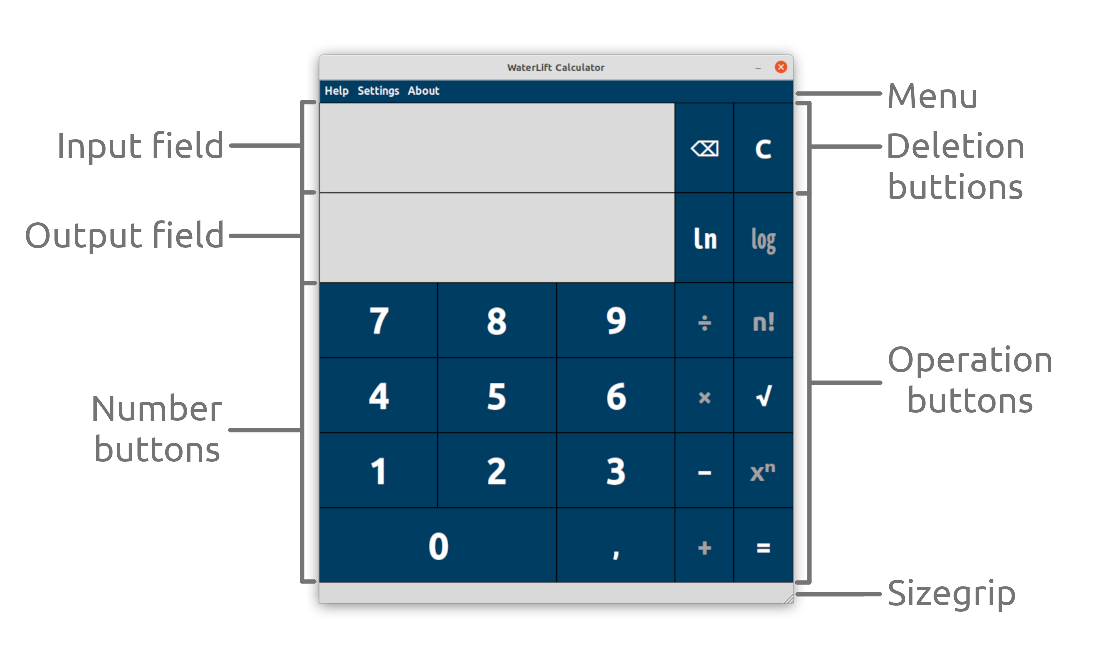
\includegraphics{user_interface01.eps}}
        \caption{Main window}
        \label{pic:UI_Main_Window_01}
    \end{figure}

\pagebreak

\section{Appearance}
    We also provide 7 color themes for your better calculating experience.
    \begin{figure}[h]
        \centering
        \scalebox{0.4}{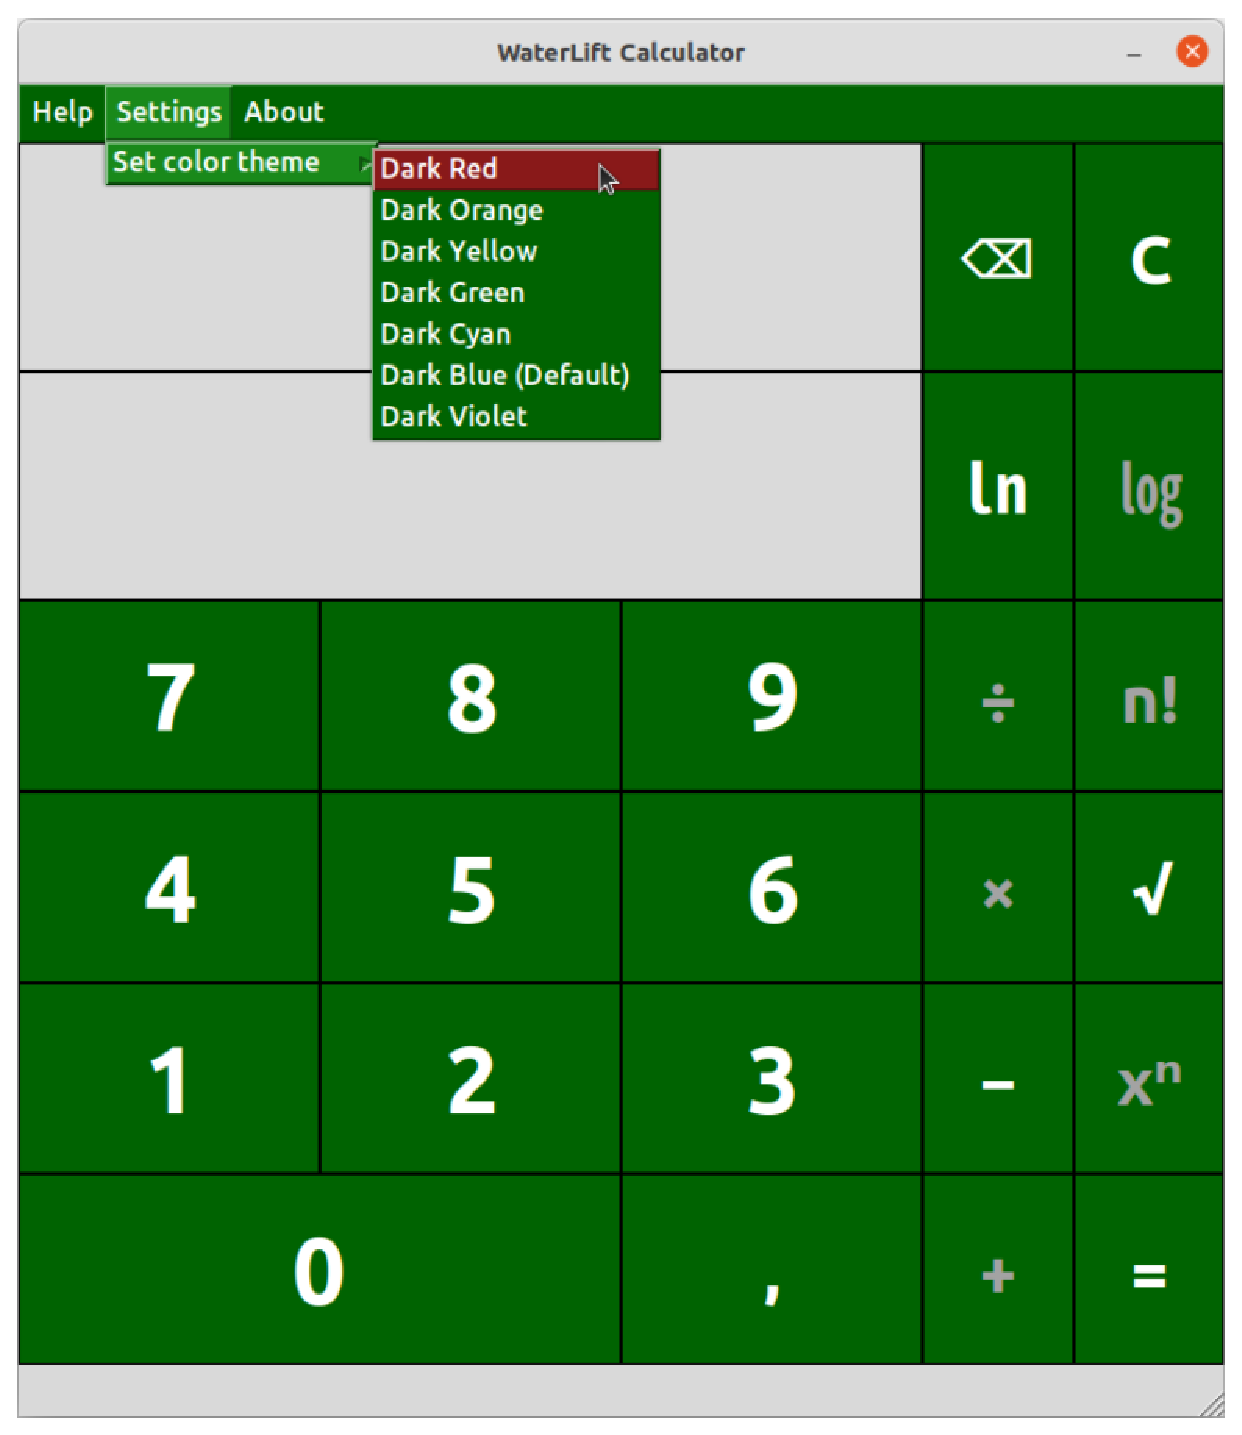
\includegraphics{user_interface02.eps}}
        \caption{Color scheme changing}
        \label{fig:UI_Main_Window_02}
    \end{figure}

\pagebreak

\section{Features}
    We have added some interesting features that can make your calculating much easier.
    \subsection{"No zero part"}
        No need to write zero in decimal numbers, the calculator add it by itself.
        \begin{figure}[h]
            \centering
            \scalebox{0.45}{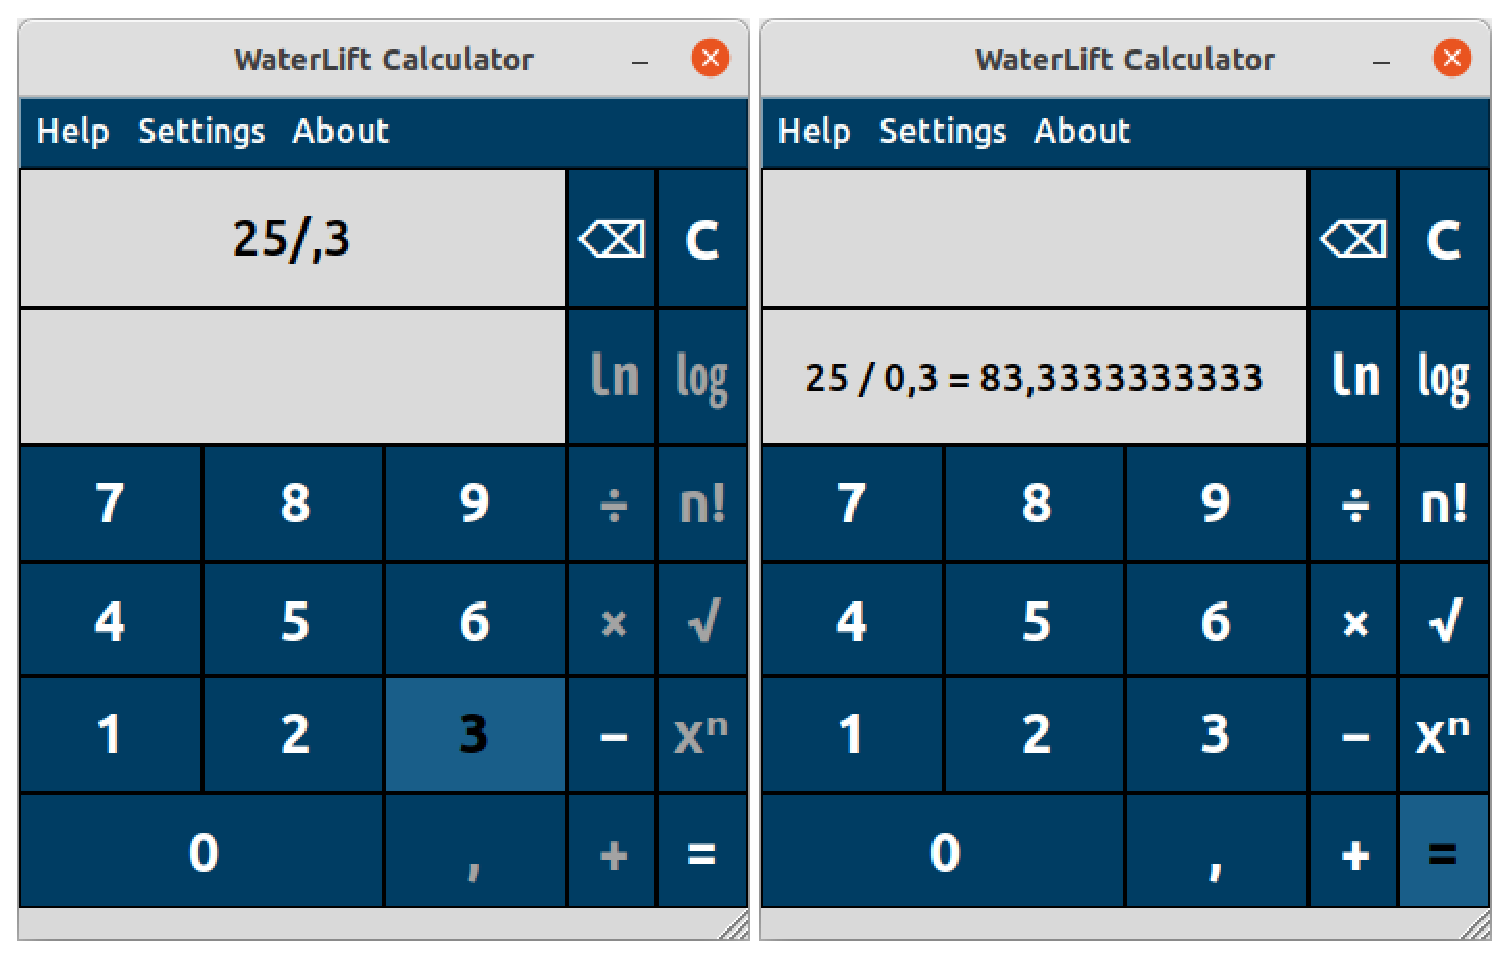
\includegraphics{no_zero_part.eps}}
            \caption{"No zero part" feature}
            \label{pic:"no_zero_part"}
        \end{figure}

    \subsection{"Continue the calculating"}
        After the evaluation of the last expression,
        \begin{itemize}
            \item press \keys{=} to put the result into the input field
            \item or press the operation sign (except \keys{√}, \keys{log}, \keys{ln}) to put the result into the input field with it.
        \end{itemize}
        \begin{figure}
            \centering
            \scalebox{0.45}{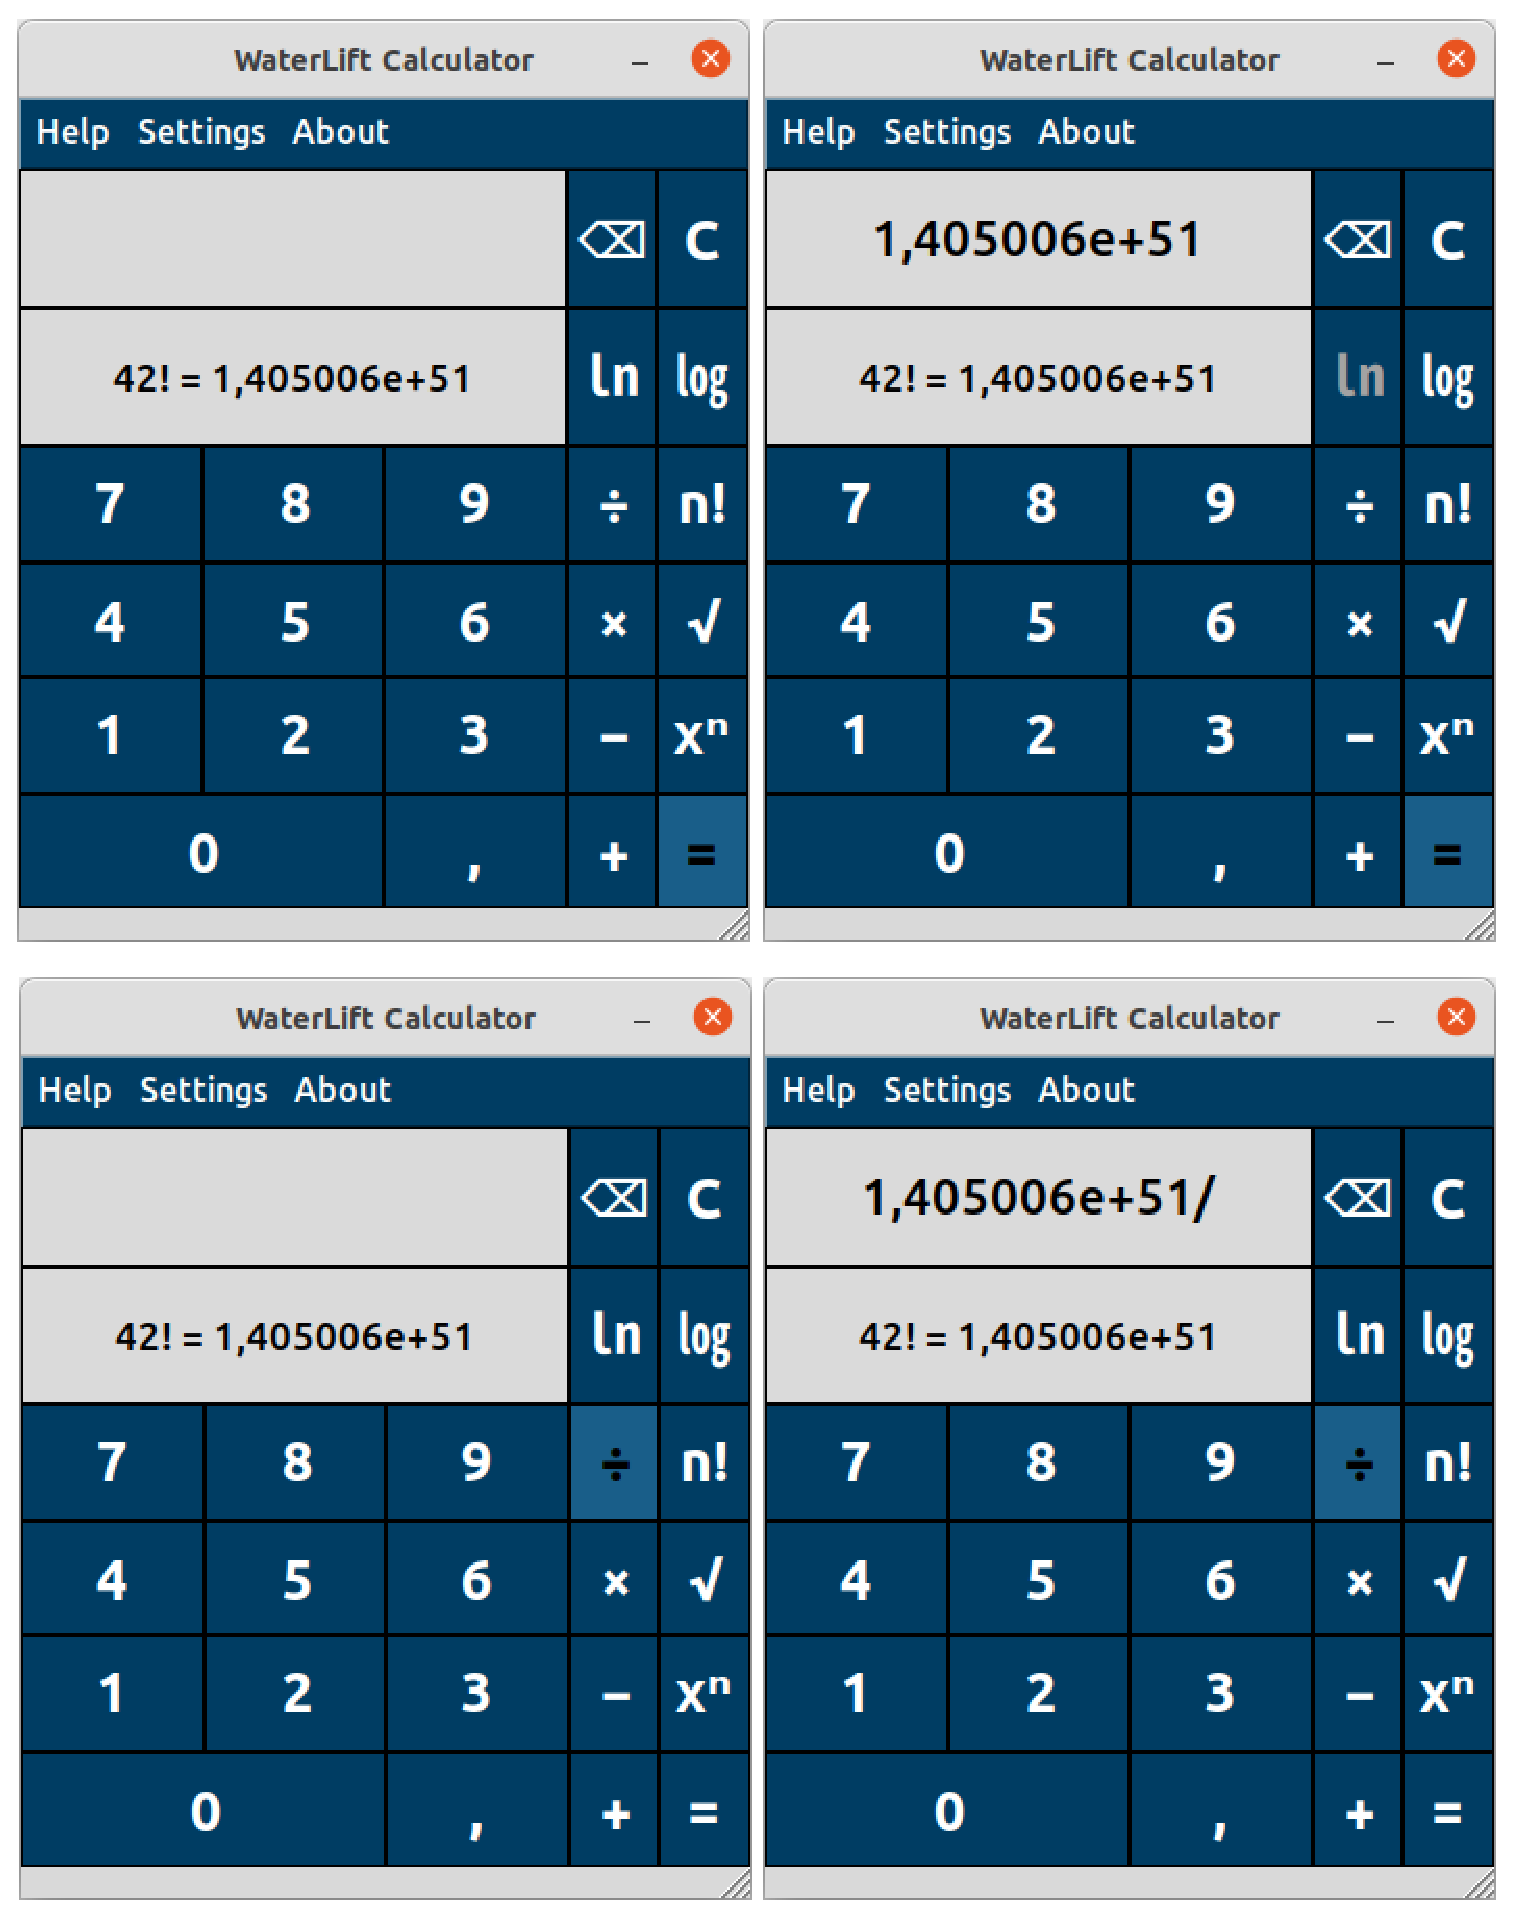
\includegraphics{continue_the_calculating01-02.eps}}
            \caption{"Continue the calculating" feature}
            \label{pic:continue_the_calculating01}
        \end{figure}

    \subsection{"Change the operation sign"}
        When you put an operation sign into the input field, you can change it by pressing another.
        \begin{figure}[h]
            \centering
            \scalebox{0.45}{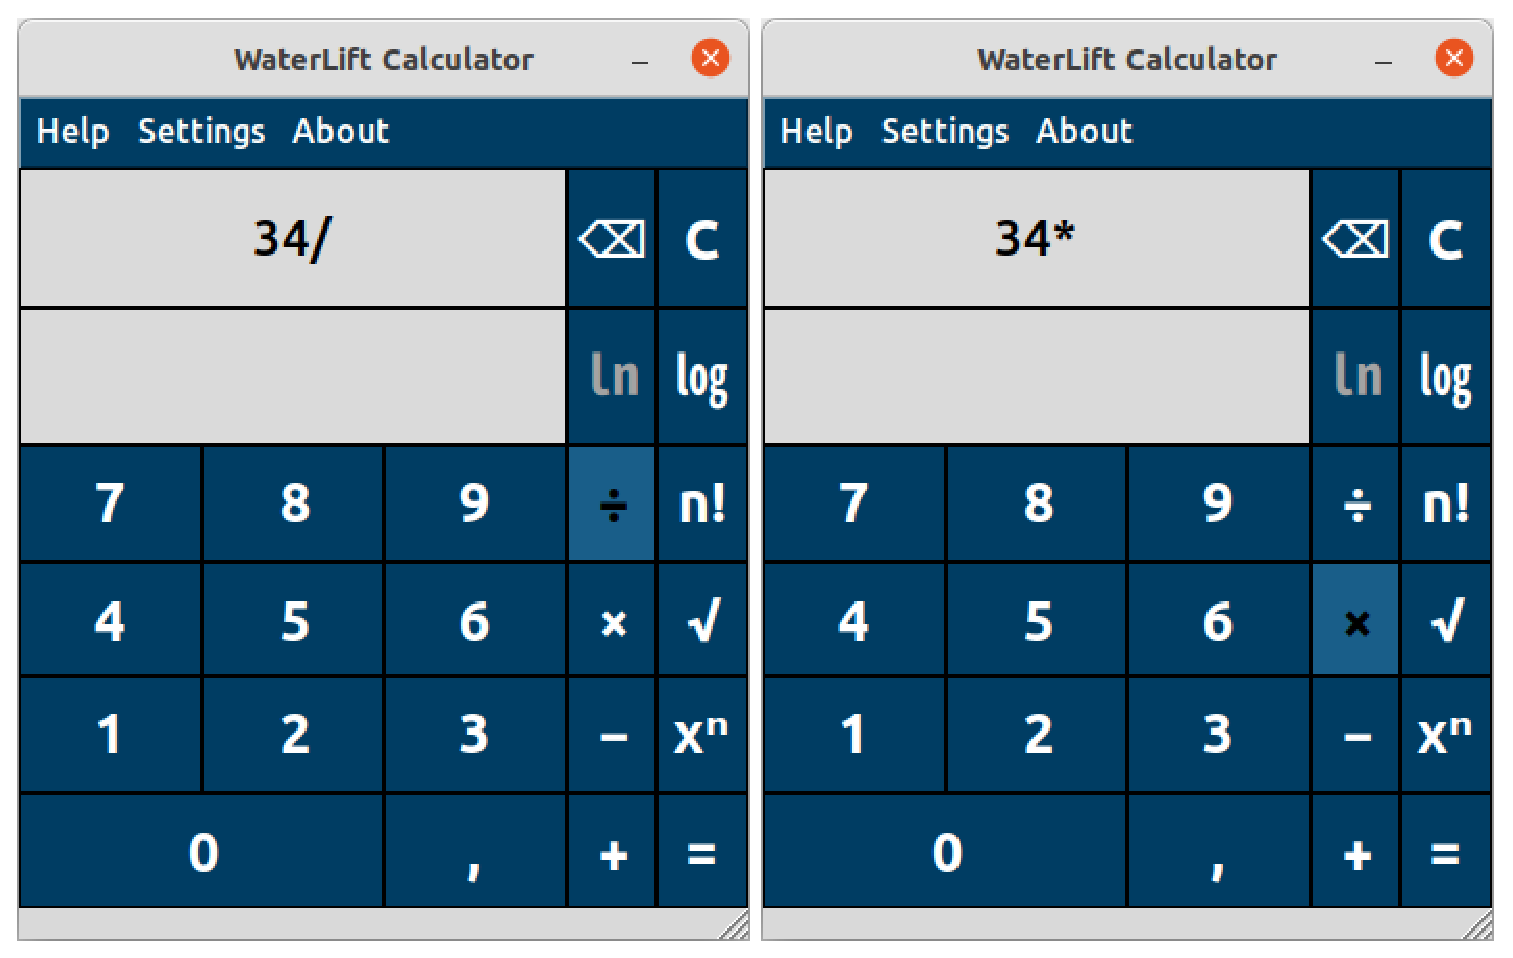
\includegraphics{change_the_operation_sign.eps}}
            \caption{"Change the operation sign" feature}
            \label{pic:change_the_operation_sign}
        \end{figure}

    \subsection{Window size control}
        You can change the window size by clicking the \keys{left mouse button} on the \emph{sizegrip} and moving the mouse.

    \subsection{Inactive buttons}
        The buttons become inactive if their using is impossible in the current expression.

    \subsection{Keyboard input support}
        We provide keyboard support for all input buttons. You can find Keyboard bindings table on the page \pageref{tab:Keyboard bindings}.

    \subsection{In-build user manual}
        You can always open a short version of this manual by clicking \keys{Help} or pressing the \keys{H} keyboard button.
        \begin{figure}[h]
            \centering
            \scalebox{0.35}{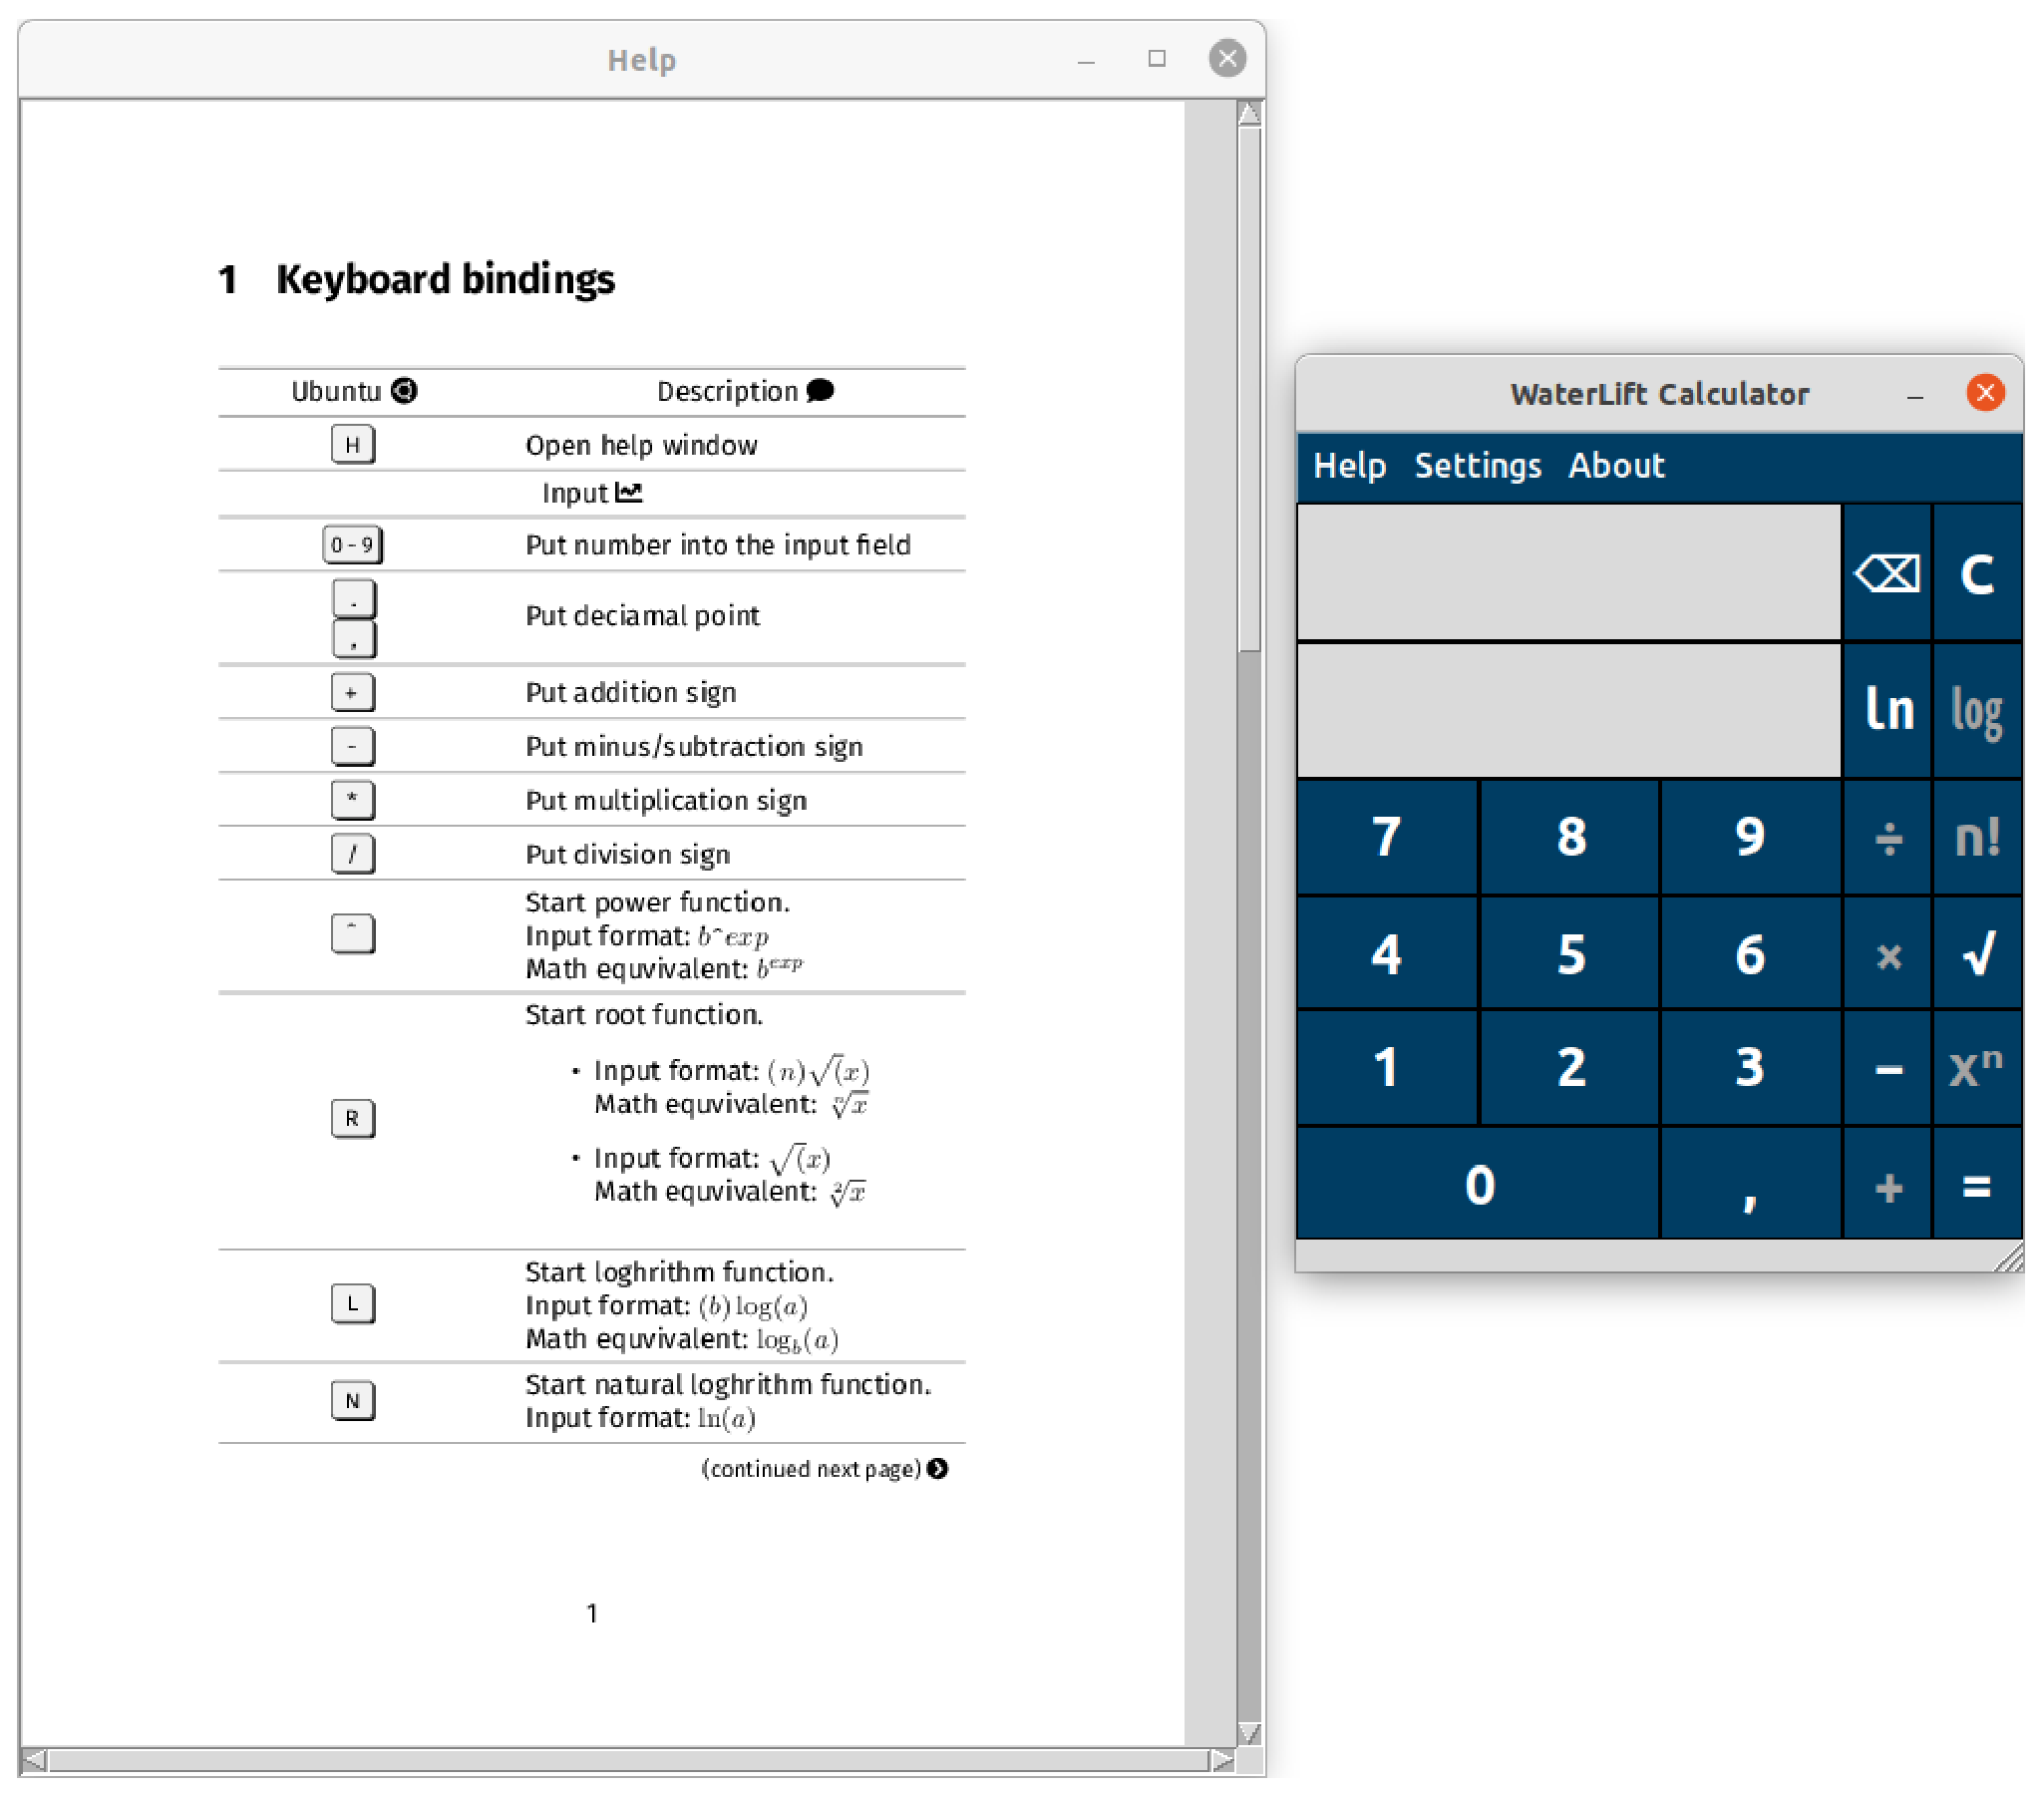
\includegraphics{help_window.eps}}
            \caption{In-build user manual}
            \label{pic:"in-build_use_manual"}
        \end{figure}

\pagebreak

\section{Operation limitations}
    \label{tab:operation_limits}
    \begin{xltabular}{\textwidth}{
        >{\setmenukeyswin}c @{\hspace{3em}} 
        >{\renewcommand\cellalign{cl}}X}
        
        \toprule
        Operation \faCalculator & \multicolumn{1}{c}{Limitation \faTimesCircle}\\
        \midrule
        \endfirsthead
        
        \footnotesize \faChevronCircleLeft\ (from previous page)\\[1em]
        \toprule
        Operation \faCalculator & \multicolumn{1}{c}{Limitation \faTimesCircle}\\
        \midrule
        \endhead
        
        \\[-0.8em]
        \multicolumn{2}{r}{\footnotesize (continued next page) \faChevronCircleRight} 
        \endfoot
        
        \bottomrule
        \endlastfoot

        \keys{\texttt{+}} & No limitation
        \\* \midrule
        
        \keys{-} & No limitation
        \\* \midrule
        
        \keys{*} & No limitation
        \\* \midrule
        
        \keys{$\div$} & $a\div b, b\neq 0$
        \\* \midrule
        
        \keys{\^{}} & $b^{exp}, exp\in \mathbb{N}$
        \\* \midrule
        
        \keys{$\sqrt{}$} & 
        \begin{itemize}[leftmargin=*]
            \item  \vspace{-2em} $\sqrt[n]{x}, n \neq 0$
            \item  $\sqrt[n]{-x}, n \in \{2n+1|n \in \mathbb{Z}\}$\vspace{-1em}
        \end{itemize}
        \\* \midrule
        
        \keys{$\log$} & $\log_{b}{a}, b>0 \wedge b\neq 1, a>0$
        \\* \midrule
        
        \keys{$\ln$} & $\ln{a}, a>0$
        \\* \midrule
        
        \keys{!} & $n!, n \in \mathbb{N}$
        \\*
    \end{xltabular}

\pagebreak

\section{Keyboard bindings}
    \label{tab:Keyboard bindings}
    \begin{xltabular}{\textwidth}{
        >{\setmenukeyswin}c @{\hspace{3em}} 
        >{\renewcommand\cellalign{cl}}X}
        
        \toprule
        Ubuntu \faUbuntu & \multicolumn{1}{c}{ Description \faComment}\\
        \midrule
        \endfirsthead
        
        \footnotesize \faChevronCircleLeft\ (from previous page)\\[1em]
        \toprule
        Ubuntu \faUbuntu & \multicolumn{1}{c}{ Description \faComment}\\
        \midrule
        \endhead
        
        \\[-0.8em]
        \multicolumn{2}{r}{\footnotesize (continued next page) \faChevronCircleRight} 
        \endfoot
        
        \bottomrule
        \endlastfoot

        \keys{H} & Open help window
        \\* \midrule
        
       \multicolumn{2}{c}{\sffamily Input \faChartLine}
        \\* \midrule
        
        \keys{0 - 9} & Put number into the input field
        \\* \midrule
        
        \makecell{%
        \keys{.}\\
        \keys{,}} & Put decimal point
        \\* \midrule
        
        \keys{\texttt{+}} & Put addition sign
        \\* \midrule
        
        \keys{-} & Put minus/subtraction sign
        \\* \midrule
        
        \keys{*} & Put multiplication sign
        \\* \midrule
        
        \keys{/} & Put division sign
        \\* \midrule
        
        \keys{\^{}} & Start power function. \newline Input format: $b\texttt{\^{}}exp$ \newline Math equivalent: $b^{exp}$
        \\* \midrule
        
        \keys{R} & Start root function.
        \begin{itemize}[leftmargin=*]
            \item  Input format: $n \sqrt x$ \newline Math equivalent: $\sqrt[n]{x}$
            \item  Input format: $\sqrt x$ \newline Math equivalent: $\sqrt[2]{x}$
        \end{itemize}
        \\* \midrule
        
        \keys{L} & Start logarithm function. \newline Input format: $(b)\log(a)$ \newline Math equivalent: $\log_b(a)$
        \\* \midrule
        
        \keys{N} & Start natural logarithm function. \newline Input format: $\ln(a)$
        \\* \midrule
        
        \keys{!} & Put factorial sign. \newline Input format: $n!$
        \\* \midrule
        
        \multicolumn{2}{c}{\sffamily Other \faKeyboard}
        \\* \midrule
        
        \makecell{%
        \keys{Enter}\\
        \keys{=}} & Evaluate the expression
        \\*
        \midrule
        
        \makecell{%
        \keys{Delete}\\
        \keys{BackSpace}} & Delete last symbol from the input field. \newline If the input field is empty, clear the output field.
        \\*
        \midrule
        
        \keys{C} & Clear the input field. \newline If the input field is empty, clear the output field.
        \\* \midrule
        
        \keys{\esc} & Close current window.\newline If was pressed on the main window, application will be closed.
        \\*
    \end{xltabular}
    
\pagebreak

\end{document}
